% !Tex root = Vorlage.tex
\newpage
\section{Execution}
A number of experiments have been conducted in order to evaluate the capabilities of empirical risk minimization (ERM) techniques for functional dependency discovery.

\subsection{FD Imputer}
The FD Imputer

\subsection{ML Imputer}

\subsubsection{Overfitting the ML Imputer}

\subsection{Comparing ML Imputer with FD Imputer}
When comparing the ML Imputer to the FD Imputer, it is necessary to explain the scope of such an comparison.
Due to the definition of a FD, the FD Imputer cannot approximate numerical values.
It allways assumes data to be classifiable.
Meanwhile, the ML Imputer is able to perform regression, predicting a continuous label for a given input.

The measure chosen to compare imputation performance on columns containing numeric values is the \emph{mean squared error} (MSE).
To compare classification performance, the F1-measure was chosen.


\subsection{Classification Performance}
ML Imputer and FD Imputer were compared on two datasets, Adult\footnote{\url{https://archive.ics.uci.edu/ml/datasets/adult}} and Nursery\footnote{\url{https://archive.ics.uci.edu/ml/datasets/nursery}}.

Figure~\ref{fig:f1_ml_fd_adult} compares the F1-scores of both ML Imputer and FD Imputer on the Adult dataset.
One can observe that for most FDs, the ML Imputer performs better than the FD Imputer.
\begin{figure}[h]
     \centering
     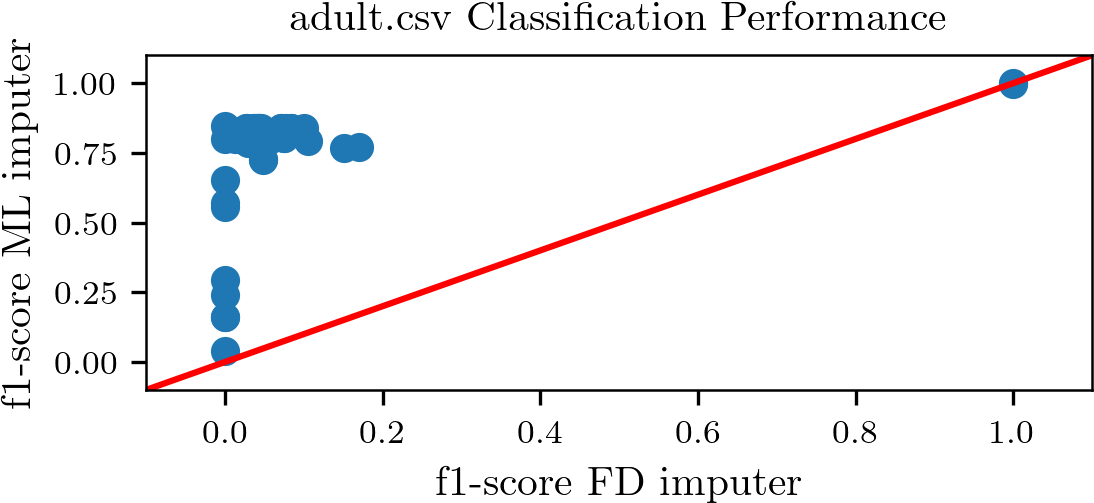
\includegraphics[width=.8\textwidth]{../figures/adult/f1_ml_fd_adult}
     \caption{The figure compares the f1-score of the FD Imputer compared to the f1-score of the ML Imputer. Each point represents one FD.}
     \label{fig:f1_ml_fd_adult}
 \end{figure}
FD Imputer performance and ML Imputer performance seem to be proportional.
If the ML imputer's F1-score is lower than 0.7, the FD Imputer's F1-score for the same FD is 0.
However, for FD's where the ML Imputer scores are larger than 0.7, the FD Imputer scores better than 0.0.
Interestingly, there are two FDs for which the FD Imputer performs equally good or better than the ML Imputer.

The same comparison as
 \begin{figure}[h]
     \centering
     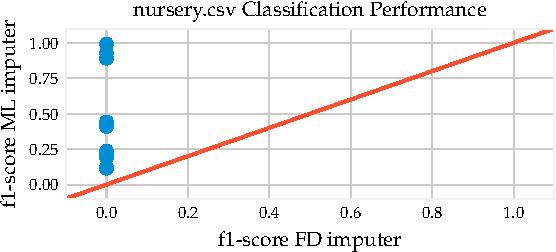
\includegraphics[width=.8\textwidth]{../figures/nursery/f1_ml_fd_nursery}
     \caption{Some ohter caption.}
     \label{fig:f1_ml_fd_nursery}
\end{figure}

\subsection{Begriffsdiskussion}
Lorem ipsum dolor sit amet, consetetur sadipscing elitr, sed diam nonumy eirmod
tempor invidunt ut labore et dolore magna aliquyam erat, sed diam voluptua. At
vero eos et accusam et justo duo dolores et ea rebum. Stet clita kasd gubergren,
no sea takimata sanctus est Lorem ipsum dolor sit amet.
